\documentclass{standalone}
\usepackage{tikz}
\usetikzlibrary{patterns, positioning}
\usepackage[sfdefault]{ClearSans} %% option 'sfdefault' activates Clear Sans as the default text font
\usepackage[T1]{fontenc}

\begin{document}
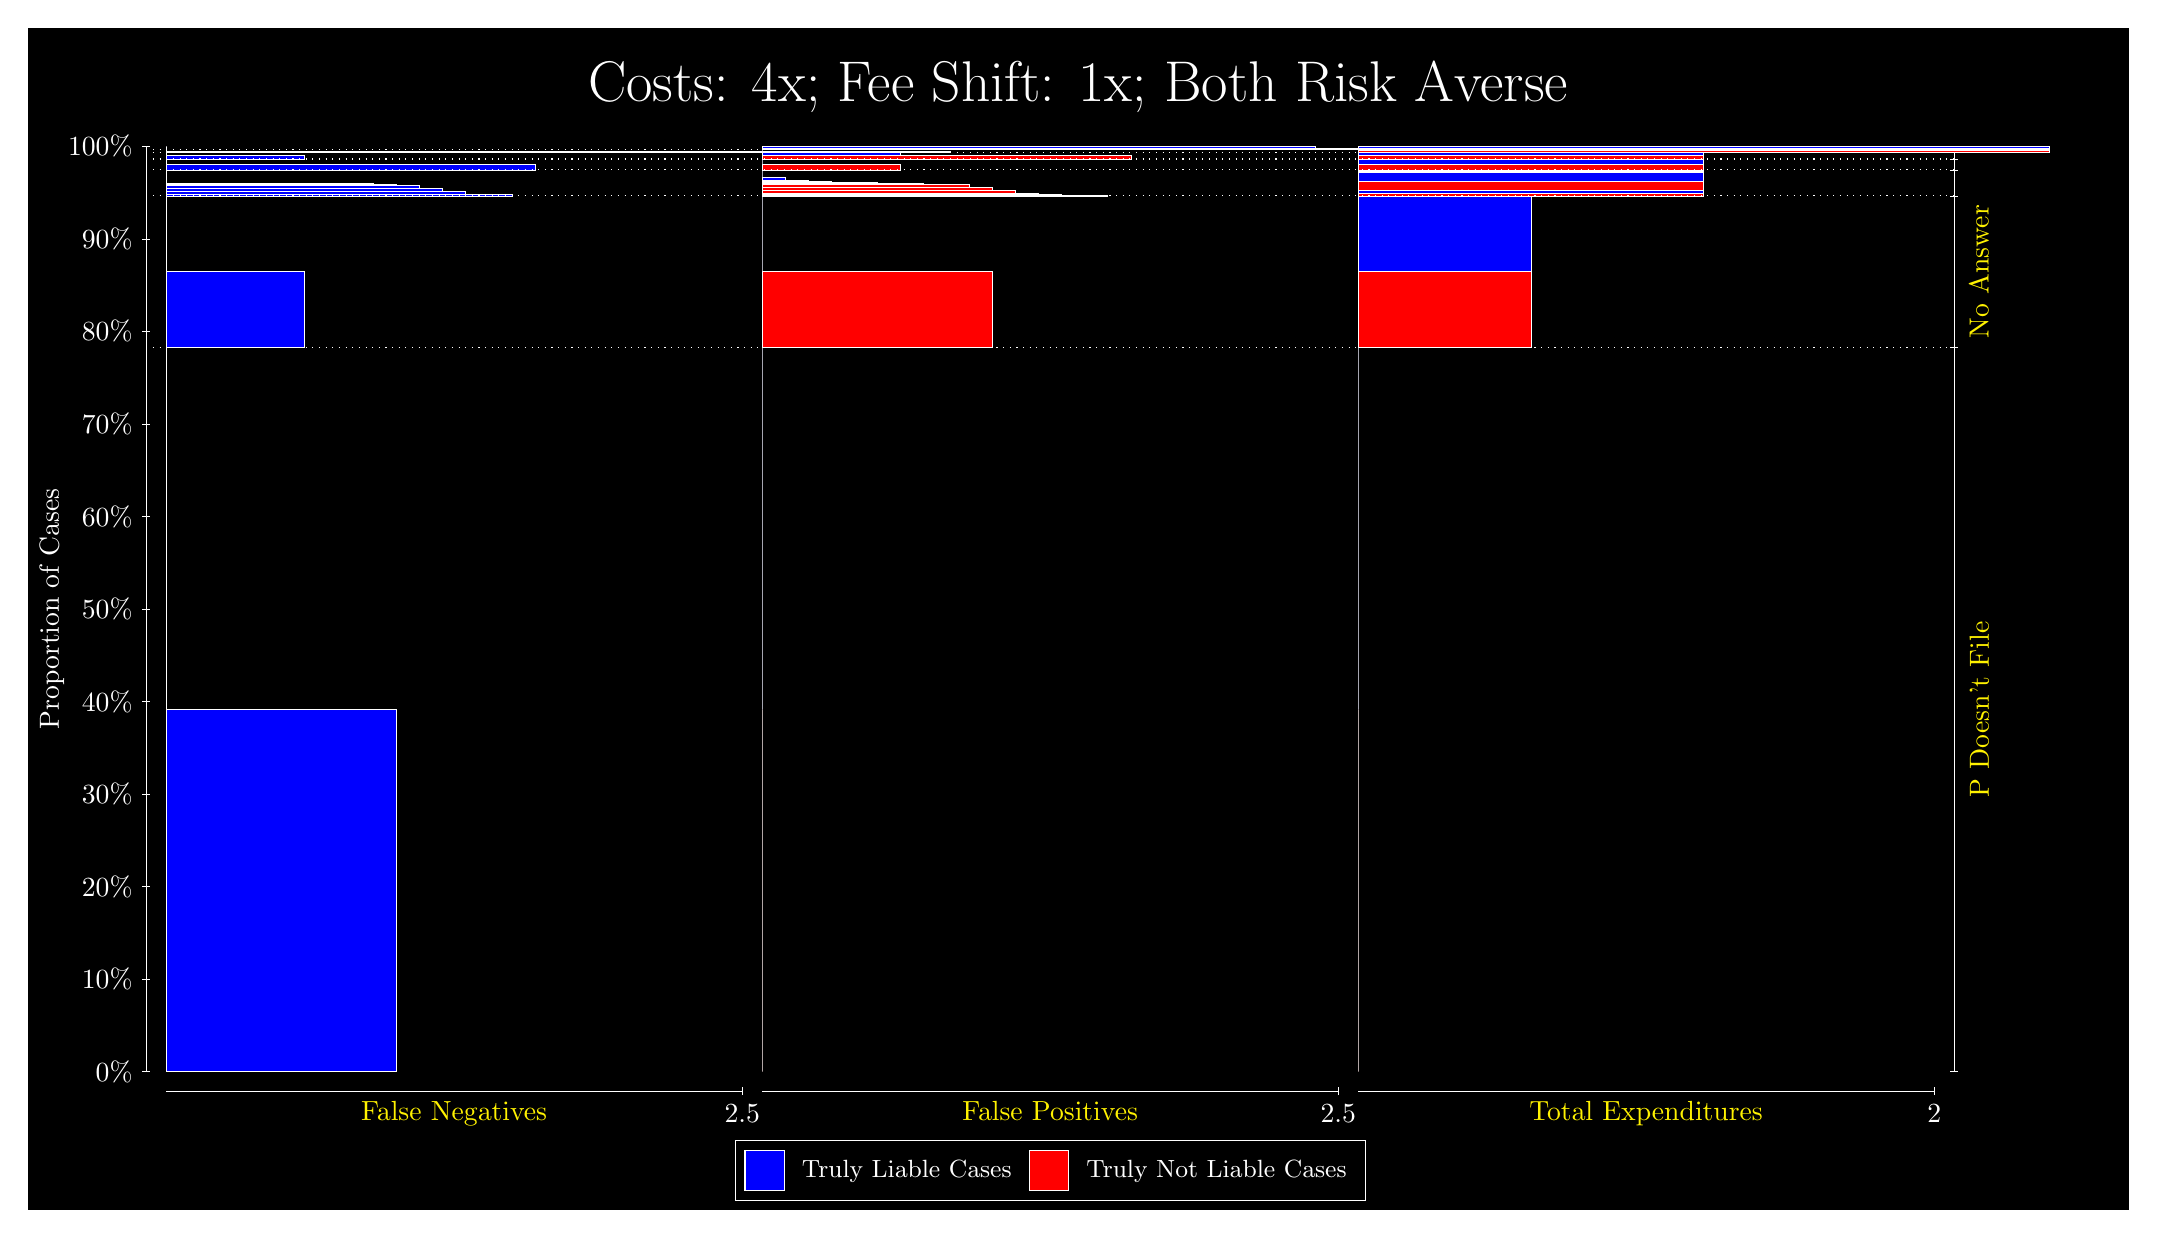
\begin{tikzpicture}
\draw[fill=black] (0,0) rectangle (26.667,15);
\draw[text=white] (0,13.5) rectangle (26.667,15) node[midway] {\huge Costs: 4x; Fee Shift: 1x; Both Risk Averse};
\draw[white, very thin] (1.5,1.75) -- (1.5,13.5);
\node[rotate=90, text=white, anchor=center] at (0.3, 7.625) {Proportion of Cases};
\draw[white, very thin] (1.45,1.75) -- (1.55,1.75);
\node[text=white, anchor=east] at (1.45, 1.75) {0\%};
\draw[white, very thin] (1.45,2.925) -- (1.55,2.925);
\node[text=white, anchor=east] at (1.45, 2.925) {10\%};
\draw[white, very thin] (1.45,4.1) -- (1.55,4.1);
\node[text=white, anchor=east] at (1.45, 4.1) {20\%};
\draw[white, very thin] (1.45,5.275) -- (1.55,5.275);
\node[text=white, anchor=east] at (1.45, 5.275) {30\%};
\draw[white, very thin] (1.45,6.45) -- (1.55,6.45);
\node[text=white, anchor=east] at (1.45, 6.45) {40\%};
\draw[white, very thin] (1.45,7.625) -- (1.55,7.625);
\node[text=white, anchor=east] at (1.45, 7.625) {50\%};
\draw[white, very thin] (1.45,8.8) -- (1.55,8.8);
\node[text=white, anchor=east] at (1.45, 8.8) {60\%};
\draw[white, very thin] (1.45,9.975) -- (1.55,9.975);
\node[text=white, anchor=east] at (1.45, 9.975) {70\%};
\draw[white, very thin] (1.45,11.15) -- (1.55,11.15);
\node[text=white, anchor=east] at (1.45, 11.15) {80\%};
\draw[white, very thin] (1.45,12.325) -- (1.55,12.325);
\node[text=white, anchor=east] at (1.45, 12.325) {90\%};
\draw[white, very thin] (1.45,13.5) -- (1.55,13.5);
\node[text=white, anchor=east] at (1.45, 13.5) {100\%};

\draw[white, very thin] (24.457,1.75) -- (24.457,13.5);
\draw[white, very thin] (24.407,1.75) -- (24.507,1.75);
\node[anchor=west] at (24.407, 1.75) {};
\draw[white, very thin] (24.407,10.95) -- (24.507,10.95);
\node[anchor=west] at (24.407, 10.95) {};
\draw[white, very thin] (24.407,12.871) -- (24.507,12.871);
\node[anchor=west] at (24.407, 12.871) {};
\draw[white, very thin] (24.407,13.201) -- (24.507,13.201);
\node[anchor=west] at (24.407, 13.201) {};
\draw[white, very thin] (24.407,13.339) -- (24.507,13.339);
\node[anchor=west] at (24.407, 13.339) {};
\draw[white, very thin] (24.407,13.423) -- (24.507,13.423);
\node[anchor=west] at (24.407, 13.423) {};
\draw[white, very thin] (24.407,13.462) -- (24.507,13.462);
\node[anchor=west] at (24.407, 13.462) {};
\draw[white, very thin] (24.407,13.5) -- (24.507,13.5);
\node[anchor=west] at (24.407, 13.5) {};

\draw[white, very thin, fill=blue] (1.75,1.75) rectangle (4.6775,6.3501);
\draw[white, very thin, fill=red] (1.75,6.3501) rectangle (1.75,10.95);
\draw[white, very thin, fill=blue] (1.75,10.95) rectangle (3.5065,11.91);
\draw[white, very thin, fill=red] (1.75,11.91) rectangle (1.75,12.871);
\draw[white, very thin, fill=blue] (1.75,12.871) rectangle (6.1413,12.886);
\draw[white, very thin, fill=blue] (1.75,12.886) rectangle (5.8486,12.894);
\draw[white, very thin, fill=blue] (1.75,12.894) rectangle (5.5558,12.927);
\draw[white, very thin, fill=blue] (1.75,12.927) rectangle (5.2631,12.966);
\draw[white, very thin, fill=blue] (1.75,12.966) rectangle (4.9703,13.002);
\draw[white, very thin, fill=blue] (1.75,13.002) rectangle (4.6775,13.017);
\draw[white, very thin, fill=blue] (1.75,13.017) rectangle (4.3848,13.027);
\draw[white, very thin, fill=blue] (1.75,13.027) rectangle (4.092,13.032);
\draw[white, very thin, fill=blue] (1.75,13.032) rectangle (3.7993,13.037);
\draw[white, very thin, fill=red] (1.75,13.037) rectangle (1.75,13.201);
\draw[white, very thin, fill=blue] (1.75,13.201) rectangle (6.4341,13.27);
\draw[white, very thin, fill=red] (1.75,13.27) rectangle (1.75,13.339);
\draw[white, very thin, fill=blue] (1.75,13.339) rectangle (3.5065,13.382);
\draw[white, very thin, fill=red] (1.75,13.382) rectangle (1.75,13.423);
\draw[white, very thin, fill=blue] (1.75,13.423) rectangle (11.704,13.441);
\draw[white, very thin, fill=red] (1.75,13.441) rectangle (1.75,13.462);
\draw[white, very thin, fill=red] (1.75,13.462) rectangle (1.75,13.479);
\draw[white, very thin, fill=blue] (1.75,13.479) rectangle (1.75,13.5);
\draw[white, very thin, fill=red] (9.3189,1.75) rectangle (9.3189,6.3501);
\draw[white, very thin, fill=blue] (9.3189,6.3501) rectangle (9.3189,10.95);
\draw[white, very thin, fill=red] (9.3189,10.95) rectangle (12.246,11.911);
\draw[white, very thin, fill=blue] (9.3189,11.911) rectangle (9.3189,12.871);
\draw[white, very thin, fill=red] (9.3189,12.871) rectangle (13.71,12.875);
\draw[white, very thin, fill=red] (9.3189,12.875) rectangle (13.417,12.88);
\draw[white, very thin, fill=red] (9.3189,12.88) rectangle (13.125,12.891);
\draw[white, very thin, fill=red] (9.3189,12.891) rectangle (12.832,12.905);
\draw[white, very thin, fill=red] (9.3189,12.905) rectangle (12.539,12.941);
\draw[white, very thin, fill=red] (9.3189,12.941) rectangle (12.246,12.979);
\draw[white, very thin, fill=red] (9.3189,12.979) rectangle (11.954,13.012);
\draw[white, very thin, fill=red] (9.3189,13.012) rectangle (11.661,13.019);
\draw[white, very thin, fill=red] (9.3189,13.019) rectangle (11.368,13.035);
\draw[white, very thin, fill=blue] (9.3189,13.035) rectangle (10.783,13.039);
\draw[white, very thin, fill=blue] (9.3189,13.039) rectangle (10.49,13.044);
\draw[white, very thin, fill=blue] (9.3189,13.044) rectangle (10.197,13.055);
\draw[white, very thin, fill=blue] (9.3189,13.055) rectangle (9.9044,13.069);
\draw[white, very thin, fill=blue] (9.3189,13.069) rectangle (9.6116,13.106);
\draw[white, very thin, fill=blue] (9.3189,13.106) rectangle (9.3189,13.201);
\draw[white, very thin, fill=red] (9.3189,13.201) rectangle (11.075,13.271);
\draw[white, very thin, fill=blue] (9.3189,13.271) rectangle (9.3189,13.339);
\draw[white, very thin, fill=red] (9.3189,13.339) rectangle (14.003,13.381);
\draw[white, very thin, fill=blue] (9.3189,13.381) rectangle (11.075,13.423);
\draw[white, very thin, fill=red] (9.3189,13.423) rectangle (9.3189,13.444);
\draw[white, very thin, fill=blue] (9.3189,13.444) rectangle (9.3189,13.462);
\draw[white, very thin, fill=red] (9.3189,13.462) rectangle (19.273,13.479);
\draw[white, very thin, fill=blue] (9.3189,13.479) rectangle (16.345,13.5);
\draw[white, very thin, fill=red] (16.888,1.75) rectangle (16.888,6.3501);
\draw[white, very thin, fill=blue] (16.888,6.3501) rectangle (16.888,10.95);
\draw[white, very thin, fill=red] (16.888,10.95) rectangle (19.083,11.911);
\draw[white, very thin, fill=blue] (16.888,11.911) rectangle (19.083,12.871);
\draw[white, very thin, fill=red] (16.888,12.871) rectangle (21.279,12.907);
\draw[white, very thin, fill=blue] (16.888,12.907) rectangle (21.279,12.944);
\draw[white, very thin, fill=red] (16.888,12.944) rectangle (21.279,13.056);
\draw[white, very thin, fill=blue] (16.888,13.056) rectangle (21.279,13.17);
\draw[white, very thin, fill=red] (16.888,13.17) rectangle (21.279,13.186);
\draw[white, very thin, fill=blue] (16.888,13.186) rectangle (21.279,13.201);
\draw[white, very thin, fill=red] (16.888,13.201) rectangle (21.279,13.271);
\draw[white, very thin, fill=blue] (16.888,13.271) rectangle (21.279,13.339);
\draw[white, very thin, fill=red] (16.888,13.339) rectangle (21.279,13.381);
\draw[white, very thin, fill=blue] (16.888,13.381) rectangle (21.279,13.423);
\draw[white, very thin, fill=red] (16.888,13.423) rectangle (25.67,13.444);
\draw[white, very thin, fill=blue] (16.888,13.444) rectangle (25.67,13.462);
\draw[white, very thin, fill=red] (16.888,13.462) rectangle (25.67,13.479);
\draw[white, very thin, fill=blue] (16.888,13.479) rectangle (25.67,13.5);
\draw[white, dotted] (1.5,10.95) -- (24.457,10.95);
\draw[white, dotted] (1.5,12.871) -- (24.457,12.871);
\draw[white, dotted] (1.5,13.201) -- (24.457,13.201);
\draw[white, dotted] (1.5,13.339) -- (24.457,13.339);
\draw[white, dotted] (1.5,13.423) -- (24.457,13.423);
\draw[white, dotted] (1.5,13.462) -- (24.457,13.462);
\draw[white, very thin] (1.75,1.5) -- (9.0689,1.5);
\node[text=yellow, anchor=north] at (5.4094, 1.5) {False Negatives};
\draw[white, very thin] (9.0689,1.45) -- (9.0689,1.55);
\node[text=white, anchor=north] at (9.0689, 1.45) {2.5};

\draw[white, very thin] (9.3189,1.5) -- (16.638,1.5);
\node[text=yellow, anchor=north] at (12.978, 1.5) {False Positives};
\draw[white, very thin] (16.638,1.45) -- (16.638,1.55);
\node[text=white, anchor=north] at (16.638, 1.45) {2.5};

\draw[white, very thin] (16.888,1.5) -- (24.207,1.5);
\node[text=yellow, anchor=north] at (20.547, 1.5) {Total Expenditures};
\draw[white, very thin] (24.207,1.45) -- (24.207,1.55);
\node[text=white, anchor=north] at (24.207, 1.45) {2};

\node[text=yellow, centered, rotate=90] at (24.777, 6.3501) {P Doesn't File};
\node[text=yellow, centered, rotate=90] at (24.777, 11.91) {No Answer};






\draw (12.978300999999998,1.5) node[draw=none] (baseCoordinate) {};
\begin{scope}[align=center]
        \matrix[scale=0.5, draw=white, below=0.5cm of baseCoordinate, nodes={draw}, column sep=0.1cm]{
            \node[rectangle, draw, minimum width=0.5cm, minimum height=0.5cm, fill=blue] {}; &
            \node[draw=none, font=\small, text=white] (B) {Truly Liable Cases}; &
            \node[rectangle, draw, minimum width=0.5cm, minimum height=0.5cm, fill=red] {}; &
            \node[draw=none, font=\small, text=white] (B) {Truly Not Liable Cases}; \\
            };
\end{scope}

\end{tikzpicture}
\end{document}